\documentclass[11pt]{article}
\usepackage[T1]{fontenc}
\usepackage{lmodern}
\usepackage{microtype}
\usepackage{amsmath,amssymb,amsthm,mathtools}
\usepackage{booktabs}
\usepackage{xcolor}
\usepackage{tikz}
\usetikzlibrary{arrows.meta}
\usepackage{enumitem}
\usepackage[hidelinks]{hyperref}
\usepackage[margin=1in]{geometry}

\newtheorem{theorem}{Theorem}[section]
\newtheorem{lemma}[theorem]{Lemma}
\newtheorem{proposition}[theorem]{Proposition}
\newtheorem{corollary}[theorem]{Corollary}
\theoremstyle{definition}
\newtheorem{definition}[theorem]{Definition}
\theoremstyle{remark}
\newtheorem{remark}[theorem]{Remark}

\newcommand{\Z}{\mathbb Z}
\newcommand{\N}{\mathbb N}
\newcommand{\Ftwo}{\mathbb F_2}
\newcommand{\vTwo}{\nu_2}
\newcommand{\abs}[1]{\lvert#1\rvert}
\newcommand{\norm}[1]{\lVert#1\rVert}
\newcommand{\bits}{\{0,1\}^2}

\title{A finite-step lattice walk in $\Z^3$ with no three collinear vertices}
\author{Erik Kalviainen}
\date{August 31, 2026}
\begin{document}
\maketitle

\begin{abstract}
We give an explicit negative answer to Erd\H{o}s Problem~193.  A nested
discrete Hilbert path $H\colon\N\to\N^2$ carries one of four terminal
orientation states.  We encode that state twice: as a Gray-code corner
appended to the planar coordinates and as a residue modulo four appended to
the height.  The resulting sequence in $\Z^3$ uses every Hilbert index, has
successive steps in one fixed finite set, and has no three collinear vertices.
The obstruction is an all-pairs two-adic identity equating a valuation of
each planar chord with the ordinary two-adic valuation of its height gap.
The complete tagged construction has also been formalized in Lean~4 against
Mathlib; the formal theorem uses no additional axioms.
\end{abstract}

\section{Introduction}

Let $S\subseteq\Z^3$ be finite.  An infinite $S$-walk is a sequence
$(P_a)_{a\geq 0}$ in $\Z^3$ such that $P_{a+1}-P_a\in S$ for every $a$.
Erd\H{o}s Problem~193 asks whether every such walk must contain three
collinear points \cite{Bloom193,GerverRamsey1979}.  Gerver and Ramsey proved
the corresponding assertion in dimension two and proved a bounded-collinearity
result in dimension three \cite{GerverRamsey1979}.

Our answer to the stated three-dimensional question is negative.

\begin{theorem}[Main theorem]\label{thm:main}
There are a finite set $S\subseteq\Z^3$ and an infinite sequence
$P\colon\N\to\Z^3$ such that
\[
  P_{a+1}-P_a\in S\qquad(a\in\N),
\]
and no three distinct terms of $P$ are collinear.
\end{theorem}

The construction uses the discrete Hilbert path, but the space-filling
property is not the decisive ingredient.  What matters is its finite-state
quadrant recursion.  For indices ending in the same state, a two-adic
valuation of the planar chord already equals the valuation of the index gap.
We remove the same-state restriction by appending the state itself as one
new binary digit in each planar coordinate and one new base-$4$ digit in the
height.

The proof has three parts:
\begin{enumerate}[nosep]
\item prove the same-terminal-state pair law for $H$;
\item use matching planar and height tags to extend it to every pair; and
\item apply the all-pairs law to a hypothetical collinear triple, then bound
      the successive tagged steps.
\end{enumerate}
Section~\ref{sec:hilbert} supplies the Hilbert decoder and its finite-state
properties.  Section~\ref{sec:pair} proves the same-state pair law.
Section~\ref{sec:tagging} constructs the tagged walk and proves its all-pairs
law.  Sections~\ref{sec:triple} and~\ref{sec:steps} finish the theorem.
Section~\ref{sec:formal} records verification and evidence, not an additional
premise of the proof.

\section{A nested discrete Hilbert path}\label{sec:hilbert}

\subsection{A four-state decoder}

On a bit pair $(x,y)\in\bits$, define the four square transformations
\[
\begin{aligned}
 I(x,y)&=(x,y),&
 S(x,y)&=(y,x),\\
 T(x,y)&=(1-y,1-x),&
 C(x,y)&=(1-x,1-y).
\end{aligned}
\]
The transformations $S$ and $T$ are commuting involutions, with
$S\circ T=T\circ S=C$.
Here $f\circ g$ denotes function composition:
$(f\circ g)(z)=f(g(z))$, so the right-hand transformation acts first.  Thus
\[
 K=\{I,S,T,C\}\cong\Ftwo^2
\]
is closed under composition.  These are exactly the states reached by the
decoder below.

Let
\[
 c_0=(0,0),\quad c_1=(0,1),\quad c_2=(1,1),\quad c_3=(1,0)
\]
be the four child positions in the basic U-shaped traversal, and set
\[
 r_0=S,\qquad r_1=I,\qquad r_2=I,\qquad r_3=T.
\]
Here $r_q\in K$ is the digit-indexed transition map selected by digit $q$;
it is not a numeric sequence.
For a length-$\ell$ base-$4$ word
$w=q_{\ell-1}\cdots q_1q_0$, read the digits from most significant to least
significant.  The mutable current state $g\in K$ starts at $g=I$.  At digit
$q_j$, emit one pair of coordinate bits and then replace the current state:
\[
 (x_j,y_j)=g(c_{q_j}),\qquad g\longleftarrow g\circ r_{q_j}.
\]
The emitted pair at digit position $j$ is used at binary place $j$:
\begin{equation}\label{eq:Hilbert-finite}
 H_\ell(w)=
 \left(\sum_{j=0}^{\ell-1}x_j2^j,\;
       \sum_{j=0}^{\ell-1}y_j2^j\right).
\end{equation}
The reading direction and the place values point in opposite directions:
the decoder processes $q_{\ell-1},q_{\ell-2},\ldots,q_0$ in that order, while
$q_j$ writes the coordinate bits at binary place $j$.  Accordingly, for two
words ``the first mismatch from the low end'' means the least $j\geq0$ for
which their digits $q_j$ differ.
After the final digit $q_0$, define $\sigma(w)$ to be the resulting value of
$g$.  Thus $g$ denotes the changing intermediate state, while $\sigma(w)$ is
its terminal value.  This value is the accumulated quadrant transformation,
not a point or an additional coordinate.

\subsection{Hilbert properties and terminal states}

\begin{lemma}[Finite-order Hilbert properties]\label{lem:finite-hilbert}
For every $\ell\geq0$, the map from length-$\ell$ base-$4$ words to
$\{0,\ldots,2^\ell-1\}^2$ given by \eqref{eq:Hilbert-finite} is a bijection.
Words representing consecutive integers map to lattice neighbors.  Moreover,
for every length-$\ell$ word $w$,
\[
 H_{\ell+2}(00w)=H_\ell(w)
 \quad\text{and}\quad
 \sigma(00w)=\sigma(w).
\]
\end{lemma}

\begin{proof}
First observe that the decoder respects its current state.  Suppose a suffix
is decoded from state $g$ instead of $I$.  If the $I$-started state at some
later digit is $h$, the other state is $g\circ h$: both update on the right by
the same $r_q$.  The emitted pair is correspondingly
$(g\circ h)(c_q)=g(h(c_q))$.  Thus the entire suffix route decoded from $g$ is
the bitwise $g$-transform of the route decoded from $I$.

Induct on $\ell$, recording simultaneously that the order-$\ell$ route starts
at $(0,0)$ and ends at $(2^\ell-1,0)$.  The claim is immediate for $\ell=0$.
Put $N=2^\ell$.  At order $\ell+1$, the first digit places four transformed
copies of the order-$\ell$ route in four disjoint $N$-by-$N$ quadrants.
Bitwise $S$ sends $(x,y)$ to $(y,x)$, while bitwise $T$ sends it to
$(N-1-y,N-1-x)$.  The four copies therefore have start--end pairs
\[
\begin{aligned}
 (0,0)&\longrightarrow(0,N-1),\\
 (0,N)&\longrightarrow(N-1,N),\\
 (N,N)&\longrightarrow(2N-1,N),\\
 (2N-1,N-1)&\longrightarrow(2N-1,0).
\end{aligned}
\]
The maps $S$ and $T$ only swap or reflect square coordinates, so they preserve
unit $\ell^1$-adjacency inside each transformed copy.  The three junction
displacements are $(0,1)$, $(1,0)$, and $(0,-1)$; they give adjacency between
copies.  The four disjoint quadrants give bijectivity, and the displayed
endpoints complete the simultaneous induction.

Finally, the first leading zero emits $(0,0)$ and changes the state from $I$
to $S$.  The second emits $S(c_0)=(0,0)$ and changes the state back to $I$.
The remaining word is therefore decoded in its original state and at its
original binary places, proving both padding identities.
\end{proof}

For $n\in\N$, write $n$ in base $4$ and prepend zero digits to any sufficiently
large even length.  Lemma~\ref{lem:finite-hilbert} makes both parts of the
following definition independent of the chosen length.

\begin{definition}\label{def:H}
The nested discrete Hilbert path $H\colon\N\to\N^2$ sends $n$ to the
finite-order point of its even-padded base-$4$ word.  Its terminal state
$\sigma(n)\in K$ is the transformation left by the same decoding.
\end{definition}

To see the infinite claims explicitly, take $m\neq n$ and choose one even
length large enough for both padded base-$4$ words.  The words are distinct,
so finite-order bijectivity gives distinct points; the padding identity
identifies those points with $H(m)$ and $H(n)$.  Thus $H$ is injective.
Likewise, represent $n$ and $n+1$ at one common even length.  Finite-order
adjacency, including across a base-$4$ carry, gives
\begin{equation}\label{eq:unit-step}
 \norm{H(n+1)-H(n)}_1=1\qquad(n\in\N).
\end{equation}

\begin{figure}[htbp]
\centering
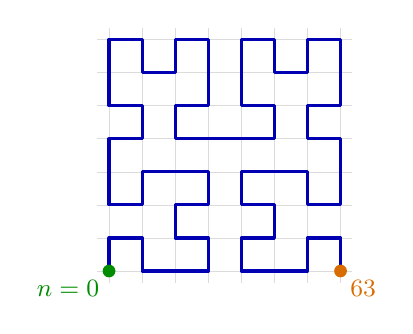
\begin{tikzpicture}[x=.42cm,y=.42cm]
 \draw[step=1,very thin,black!14] (-.35,-.35) grid (7.35,7.35);
 \draw[blue!70!black,line width=1.15pt,line cap=round,line join=round]
  (0,0)--(0,1)--(1,1)--(1,0)--(2,0)--(3,0)--(3,1)--(2,1)
  --(2,2)--(3,2)--(3,3)--(2,3)--(1,3)--(1,2)--(0,2)--(0,3)
  --(0,4)--(1,4)--(1,5)--(0,5)--(0,6)--(0,7)--(1,7)--(1,6)
  --(2,6)--(2,7)--(3,7)--(3,6)--(3,5)--(2,5)--(2,4)--(3,4)
  --(4,4)--(5,4)--(5,5)--(4,5)--(4,6)--(4,7)--(5,7)--(5,6)
  --(6,6)--(6,7)--(7,7)--(7,6)--(7,5)--(6,5)--(6,4)--(7,4)
  --(7,3)--(7,2)--(6,2)--(6,3)--(5,3)--(4,3)--(4,2)--(5,2)
  --(5,1)--(4,1)--(4,0)--(5,0)--(6,0)--(6,1)--(7,1)--(7,0);
 \fill[green!55!black] (0,0) circle (2.3pt)
  node[below left,font=\small] {$n=0$};
 \fill[orange!85!black] (7,0) circle (2.3pt)
  node[below right,font=\small] {$63$};
\end{tikzpicture}
\caption{The order-three Hilbert route.  Each segment is one planar lattice
step; the same four-copy rule produces every higher order.}
\label{fig:hilbert-trace}
\end{figure}

Only digits $0$ and $3$ alter the state.  Since $S$ and $T$ commute and each
undoes itself, for every finite word $w$,
\begin{equation}\label{eq:sigma-word}
 \sigma(w)=S^{N_0(w)\bmod2}T^{N_3(w)\bmod2},
\end{equation}
where $N_0(w)$ and $N_3(w)$ count its zero and three digits.  Thus the
terminal state remembers precisely the parities of those two counts.

For later use, every transition $g\mapsto g\circ r_q$ is invertible.  If $h$
is the outgoing state after digit $q$, then the incoming state was
$h\circ r_q$, because $r_q$ is an involution.  Moreover $r_q(c_q)=c_q$, so
the emitted pair can be recovered backwards as
\begin{equation}\label{eq:backward-emission}
 (h\circ r_q)(c_q)=h\bigl(r_q(c_q)\bigr)=h(c_q).
\end{equation}
This is the mechanism behind the pair law.


\section{The two-adic pair law}\label{sec:pair}

For a nonzero planar chord $u$, remove its largest common power of two.
The quantity $V(u)$ records twice that binary scale, plus one exactly when
both remaining coordinates are odd.  Equivalently, it distinguishes the two
possible first appearances of the chord: one coordinate becomes nonzero at
that scale, or both do.

Formally, put $\vTwo(0)=\infty$.  For
$u=(u_x,u_y)\in\Z^2\setminus\{0\}$, define
\begin{align}
 p(u)&=\min\{\vTwo(u_x),\vTwo(u_y)\},\\
 \epsilon(u)&=
 \begin{cases}
 1,&\vTwo(u_x)=\vTwo(u_y),\\
 0,&\vTwo(u_x)\neq\vTwo(u_y),
 \end{cases}\\
 V(u)&=2p(u)+\epsilon(u).\label{eq:V}
\end{align}

\begin{lemma}[Scaling]\label{lem:scaling}
For $u\neq0$ and every positive integer $k$,
\[
 V(ku)=V(u)+2\vTwo(k).
\]
\end{lemma}

\begin{proof}
Multiplication by $k$ adds $\vTwo(k)$ to each finite coordinate valuation.
It therefore adds $\vTwo(k)$ to $p(u)$ and leaves the equality bit
$\epsilon(u)$ unchanged.
\end{proof}
The factor $2$ has a concrete meaning.  Multiplication by $2$ shifts both
coordinate bit streams one place, while $V$ reserves the two consecutive
values $2j$ and $2j+1$ for the one-coordinate and two-coordinate appearances
at scale $j$.  A shift of one scale must therefore add two to $V$.

\begin{lemma}[First mismatch]\label{lem:mismatch}
Let $q_{\ell-1}\cdots q_0$ and $q'_{\ell-1}\cdots q'_0$ be equally long,
even-padded base-$4$ words with the same terminal state, and let
\[
 j=\min\{k\geq0:q_k\neq q'_k\}.
\]
Thus positions $0,\ldots,j-1$ form their common low suffix.  Their Hilbert
coordinates agree below binary place $j$.  At place $j$, exactly one
coordinate bit differs when $q_j-q'_j$ is odd, and both coordinate bits
differ when $q_j-q'_j\equiv2\pmod4$.
\end{lemma}

\begin{proof}
The words have one common low-digit suffix.  Start from their equal terminal
states and undo that suffix in lockstep.  Invertibility of every transition
shows that immediately after the mismatching digit both decoders have one
common state $h$.

Let the mismatching digits be $d\neq e$.  Their incoming states were
$h\circ r_d$ and $h\circ r_e$.  By
\eqref{eq:backward-emission}, the emitted pairs at the mismatch are
$h(c_d)$ and $h(c_e)$.  The corners $c_0,c_1,c_2,c_3$ form a cyclic Gray
code: $c_d$ and $c_e$ differ in exactly one coordinate when $d-e$ is odd,
and in both coordinates when $d-e\equiv2\pmod4$.  Every $h\in K$ only swaps
coordinates and complements coordinate bits.  It therefore permutes which
coordinates differ but preserves whether the number of differing coordinates
is one or two.  Starting from the common state $h$, the identical lower suffix
also emits identical bits below place $j$.
\end{proof}
\begin{figure}[htbp]
\centering
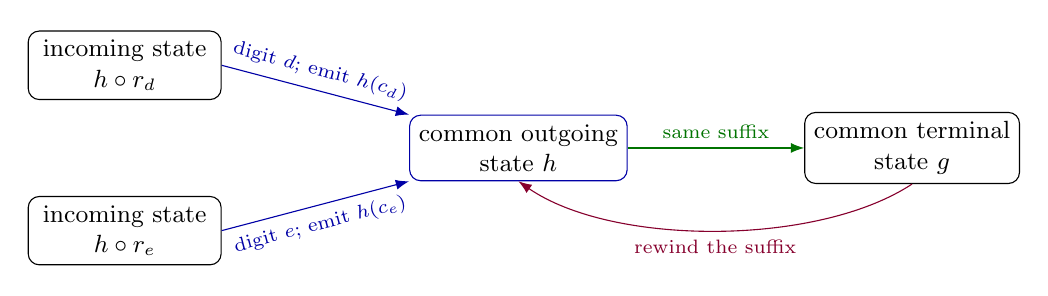
\begin{tikzpicture}[
  >=Latex,
  statebox/.style={draw,rounded corners,align=center,minimum width=2.45cm,
                   minimum height=.8cm,font=\small}
]
 \node[statebox] (ind) at (0,1.05) {incoming state\\$h\circ r_d$};
 \node[statebox] (ine) at (0,-1.05) {incoming state\\$h\circ r_e$};
 \node[statebox,draw=blue!65!black] (h) at (5,0)
       {common outgoing\\state $h$};
 \node[statebox] (g) at (10,0) {common terminal\\state $g$};
 \draw[-{Latex},blue!65!black] (ind.east) --
   node[midway,above,sloped,font=\scriptsize]
        {digit $d$; emit $h(c_d)$} (h.north west);
 \draw[-{Latex},blue!65!black] (ine.east) --
   node[midway,below,sloped,font=\scriptsize]
        {digit $e$; emit $h(c_e)$} (h.south west);
 \draw[-{Latex},green!45!black] (h.east) --
   node[midway,above,font=\scriptsize]
        {same suffix} (g.west);
 \draw[-{Latex},purple!70!black]
   (g.south) .. controls (8.8,-1.25) and (6.2,-1.25) ..
   node[midway,below,font=\scriptsize]{rewind the suffix} (h.south);
\end{tikzpicture}
\caption{The first-mismatch alignment.  Forward decoding sends the two
possibly different incoming states through digits $d$ and $e$ to one common
outgoing state $h$.  Equal terminal states let the shared low suffix be
rewound from $g$ back to $h$; rewinding changes state, not emitted bits.}
\label{fig:first-mismatch}
\end{figure}

\begin{theorem}[Same-terminal-state pair law]\label{thm:pair-law}
If $m\neq n$ and $\sigma(m)=\sigma(n)$, then
\begin{equation}\label{eq:pair-law}
 V\bigl(H(n)-H(m)\bigr)=\vTwo(\abs{n-m}).
\end{equation}
\end{theorem}

\begin{proof}
By symmetry assume $m<n$.  Pad both base-$4$ words to one common even length,
writing the digits of $m$ as $q_{\ell-1}\cdots q_0$ and those of $n$ as
$q'_{\ell-1}\cdots q'_0$.  Let $j$ be their first differing position from
the low end, and put $d=q_j$ and $e=q'_j$.  Then $d\neq e$ and
\[
 n-m=4^jM,\qquad M\equiv e-d\pmod4.
\]
If $e-d$ is odd, then $\vTwo(n-m)=2j$.  By
Lemma~\ref{lem:mismatch}, exactly one coordinate of $H(n)-H(m)$ has differing
bits at position $j$; in that coordinate the difference has the form
\[
 \pm2^j+2^{j+1}L=2^j(\pm1+2L)
\]
for some integer $L$.  The bracket is odd, so higher binary places cannot
cancel the mismatch or add another factor of two.  The other coordinate has
larger valuation.  Thus $p=j$, $\epsilon=0$, and $V=2j$.

If $e-d\equiv2\pmod4$, then $\vTwo(n-m)=2j+1$.  The same odd-bracket
calculation applies to both coordinate differences, so both have valuation
$j$.  Hence $p=j$, $\epsilon=1$, and $V=2j+1$.  These cases exhaust unequal
base-$4$ digits.
\end{proof}

\section{Tagging all four terminal states}\label{sec:tagging}

The pair law compares indices with one common terminal state.  We remove
that restriction by recording the state in one additional planar bit pair
and in the corresponding residue modulo four.  Label the four states in
cyclic order by
\[
 \lambda(I)=0,\qquad \lambda(S)=1,\qquad
 \lambda(C)=2,\qquad \lambda(T)=3,
\]
and give $g\in K$ the Gray-code corner tag
\[
 u_g=c_{\lambda(g)}.
\]
Thus
\[
\begin{array}{c|cccc}
g&I&S&C&T\\ \hline
\lambda(g)&0&1&2&3\\
u_g&(0,0)&(0,1)&(1,1)&(1,0).
\end{array}
\]
Define
\begin{equation}\label{eq:tagged-walk}
\begin{aligned}
 G(n)&=2H(n)+u_{\sigma(n)}\in\Z^2,\\
 z(n)&=4n+\lambda(\sigma(n))\in\Z,\\
 P_n&=(G(n),z(n))\in\Z^3.
\end{aligned}
\end{equation}
Multiplication by two leaves one low binary place for the planar corner tag,
while multiplication by four leaves one low base-$4$ place for the height
label.

\begin{theorem}[All-pairs tagged law]\label{thm:all-pairs}
For all distinct $m,n\in\N$, the planar chord is nonzero and
\begin{equation}\label{eq:all-pairs}
 V\bigl(G(n)-G(m)\bigr)=\vTwo\bigl(\abs{z(n)-z(m)}\bigr).
\end{equation}
\end{theorem}

\begin{proof}
Put
\[
 d=n-m,\qquad i=\lambda(\sigma(m)),\qquad
 j=\lambda(\sigma(n)),\qquad X=H(n)-H(m).
\]
Then
\begin{equation}\label{eq:tagged-chords}
 G(n)-G(m)=2X+c_j-c_i,\qquad z(n)-z(m)=4d+j-i.
\end{equation}
If $i=j$, the states agree and the corner tags cancel.  Theorem
\ref{thm:pair-law} and Lemma~\ref{lem:scaling} give
\[
 V(2X)=V(X)+2=\vTwo(\abs d)+2=\vTwo(\abs{4d}).
\]

Suppose $i\ne j$.  If $j-i$ is odd, then $c_i$ and $c_j$ are adjacent
corners in the cyclic Gray code.  Exactly one coordinate of
$2X+c_j-c_i$ is odd, so this chord is nonzero and has $V=0$.  The integer
$4d+j-i$ is also odd.

The remaining case is $j-i=\pm2$.  The two corners are opposite, so both
coordinates of $2X+c_j-c_i$ are odd.  Hence $p=0$, $\epsilon=1$, and
$V=1$.  Also
\[
 4d+j-i=4d\pm2=2(2d\pm1)
\]
has valuation one.  These cases prove \eqref{eq:all-pairs}.
\end{proof}

\section{Excluding collinear triples}\label{sec:triple}

\begin{theorem}[The tagged lift is triple-free]
\label{thm:tagged-triple-free}
The sequence $(P_n)_{n\geq0}$ in \eqref{eq:tagged-walk} contains no three
collinear terms.
\end{theorem}

\begin{proof}
Because $\lambda$ takes values in $\{0,1,2,3\}$,
\begin{equation}\label{eq:height-step}
 1\le z(n+1)-z(n)
   =4+\lambda(\sigma(n+1))-\lambda(\sigma(n))\le7.
\end{equation}
Thus $z$ is strictly increasing.  Suppose for contradiction that
$a<b<c$ and $P_a,P_b,P_c$ are collinear.  Write the adjacent height gaps
and planar chords as
\[
\begin{aligned}
 A&=z(b)-z(a),& B&=z(c)-z(b),\\
 X&=G(b)-G(a),& Y&=G(c)-G(b).
\end{aligned}
\]
Both $A$ and $B$ are positive.  Collinearity makes the full displacements
$(X,A)$ and $(Y,B)$ proportional, and their last coordinates force
\begin{equation}\label{eq:scaled-chords}
 BX=AY.
\end{equation}
Write
\[
 A=gr,\qquad B=gs,\qquad
 g=\gcd(A,B),\qquad \gcd(r,s)=1.
\]
After cancelling $g$, equation~\eqref{eq:scaled-chords} becomes $sX=rY$.
Coordinatewise coprimality gives an integer vector $W$ such that
\begin{equation}\label{eq:common-vector}
 X=rW,\qquad Y=sW.
\end{equation}
Theorem~\ref{thm:all-pairs} gives $X\ne0$, hence $W\ne0$.

Apply the all-pairs law and scaling lemma to the two adjacent pairs:
\begin{align*}
 \vTwo(g)+\vTwo(r)
  &=V(X)=V(W)+2\vTwo(r),\\
 \vTwo(g)+\vTwo(s)
  &=V(Y)=V(W)+2\vTwo(s).
\end{align*}
Therefore $\vTwo(r)=\vTwo(s)$.  Coprimality forces both valuations to be
zero, so $r$ and $s$ are odd, and either equality gives
$V(W)=\vTwo(g)$.

For the endpoint pair, the height gap is $A+B=g(r+s)$ and the planar chord
is $X+Y=(r+s)W$.  If $t=\vTwo(r+s)$, the all-pairs law gives
\[
 \vTwo(g)+t
 =V((r+s)W)
 =V(W)+2t
 =\vTwo(g)+2t.
\]
Thus $t=0$, so $r+s$ is odd.  But $r$ and $s$ are both odd, making their
sum even.  This contradiction proves the theorem.
\end{proof}

\section{The finite step menu}\label{sec:steps}

For one successive step, \eqref{eq:tagged-walk} gives
\[
\begin{aligned}
 G(n+1)-G(n)
 &=2\bigl(H(n+1)-H(n)\bigr)
   +u_{\sigma(n+1)}-u_{\sigma(n)},\\
 z(n+1)-z(n)
 &=4+\lambda(\sigma(n+1))-\lambda(\sigma(n)).
\end{aligned}
\]
The first planar term is twice a coordinate unit vector by
\eqref{eq:unit-step}; each coordinate of the tag difference lies between
$-1$ and $1$.  Equation~\eqref{eq:height-step} bounds the last coordinate.
Every successive displacement therefore belongs to the fixed finite set
\begin{equation}\label{eq:menu}
 S=\{(d_x,d_y,d_z)\in\Z^3:
       \abs{d_x}\le3,\ \abs{d_y}\le3,\ 1\le d_z\le7\}.
\end{equation}
The strictly increasing height makes $(P_n)$ infinite with no repeated
terms, and Theorem~\ref{thm:tagged-triple-free} excludes collinear triples.
This proves Theorem~\ref{thm:main}.

\section{Verification and evidence}\label{sec:formal}

\noindent\textbf{Proof boundary.}
The proof of Theorem~\ref{thm:main} ends above.  Nothing in this section is an
additional premise; it records formal verification and the status of external
claims.

\subsection{Lean formalization}

The repository \cite{Repository} contains a Lean~4 formalization in
\path{formal/Hilbert193}.  It uses Lean~4.33.0 and the corresponding pinned
Mathlib revision.  The final theorem is
\path{Hilbert193.erdos193_unconditional} in
\path{Hilbert193/Continuity.lean}.  It constructs:
\begin{enumerate}[nosep]
\item a finite set of integer three-dimensional step vectors;
\item an explicit sequence $\N\to\Z^3$ whose successive displacements lie in
      that set; and
\item a proof that every ordered triple of distinct indices fails the exact
      integer collinearity equations.
\end{enumerate}
The Lean predicate packages collinearity as the two integer
cross-multiplication equalities forced by the strictly increasing third
coordinate.  As shown in the proof above, this is the denominator-free form
of ordinary real affine collinearity for the ordered points in this walk.

The axiom audit in \texttt{Hilbert193/AxiomAudit.lean} reports only
\texttt{propext}, \texttt{Classical.choice}, and \texttt{Quot.sound}, the
standard axioms used by Mathlib.  No theorem in the construction depends on a
finite computation.  From the repository root, the formal proof is checked by
\begin{verbatim}
cd formal/Hilbert193
lake build
lake env lean Hilbert193/AxiomAudit.lean
\end{verbatim}

\subsection{Finite implementation check}

The standalone script
\path{viz/hilbert_walk_tagged_demo.py} independently evaluates the decoder,
constructs a finite tagged prefix, and checks the all-pairs identity, the
step bounds, and every collinear triple in that prefix using exact integer
arithmetic.  This is an implementation check only; no finite computation
proves the infinite theorem.

\subsection{Logical and historical status}

The theorem above is unconditional.  The Lean development checks the complete
tagged construction, while the standalone script checks an implementation
and a finite prefix only.
Novelty, priority, and correspondence with the intended
reading of Erd\H{o}s Problem~193 remain subject to external mathematical
review and community acceptance.

\section*{Acknowledgments and disclosure}

Stijn Cambie suggested the state-tagging refinement that removes the
same-terminal-state selector and shared a GPT-assisted alternative draft.
The author thanks him for this substantial simplification.

The working stack included Pi (\url{https://pi.dev/}), Oh My Pi
(\url{https://omp.sh/}), Paseo (\url{https://paseo.sh/}), and OpenAI GPT-5.6
for proof exploration, Lean code drafting, computational verification tooling,
visualization, and manuscript preparation.
The author directed the work, checked the generated artifacts, and takes
responsibility for every claim.  The proof is kernel-checked, but at the date
of this preprint it has not yet completed external mathematical peer review.

\begin{thebibliography}{9}

\bibitem{Bloom193}
T.~F. Bloom,
\newblock Erd\H{o}s Problem \#193,
\newblock \url{https://www.erdosproblems.com/193}, accessed August 19, 2026.

\bibitem{GerverRamsey1979}
J.~L. Gerver and L.~T. Ramsey,
\newblock On certain sequences of lattice points,
\newblock \emph{Pacific Journal of Mathematics} \textbf{83} (1979), no.~2,
357--363.
\newblock \url{https://doi.org/10.2140/pjm.1979.83.357}.

\bibitem{Hilbert1891}
D.~Hilbert,
\newblock \"Uber die stetige Abbildung einer Linie auf ein Fl\"achenst\"uck,
\newblock \emph{Mathematische Annalen} \textbf{38} (1891), 459--460.

\bibitem{Lean4}
L.~de Moura and S.~Ullrich,
\newblock The Lean 4 theorem prover and programming language,
\newblock in \emph{Automated Deduction---CADE 28}, Lecture Notes in Computer
Science 12699, Springer, 2021, 625--635.

\bibitem{Mathlib}
The Mathlib Community,
\newblock The Lean mathematical library,
\newblock in \emph{Proceedings of the 9th ACM SIGPLAN International Conference
on Certified Programs and Proofs}, 2020, 367--381.

\bibitem{Repository}
E.~Kalviainen,
\newblock Erd\H{o}s 193: state-tagged Hilbert lift, source code and formal
proof,
\newblock \url{https://github.com/ekalvi/erdos-193}, 2026.

\bibitem{Sagan1994}
H.~Sagan,
\newblock \emph{Space-Filling Curves},
\newblock Springer, 1994.

\end{thebibliography}

\end{document}
